\section{Das elektrische Feld I}
\begin{flushleft}
\subsection{Definition: Elektrische Ladung}
Diskrete \textbf{Ladungsverteilung} (nicht kontinuierliche)\\
Die \textbf{elektrische Ladung} ist quantifiziert, d.h sie tritt als ganzzahliges vielfaches von $\textbf{e}$ auf
\[
    e \approx 1.602 \cdot 10^{-19} \ \text{C} \: [Coulomb]
\]\[
	-e \: \hat{=} \ \text{Ladung eines Elektrons}
\]\[
	e \: \hat{=} \ \text{Ladung eines Protons}
\]
Bei allen Prozessen ist die Gesamtladung vor \& nach der Wechselwirkung identisch

\subsection{Definition Elektrische Leiter \& nicht Leiter}
\textbf{Elektrische Leiter:} Stoffe, in denen sich ein Teil der Elektronen frei bewegen kann. \\
\textbf{Nichtleiter/Isolatoren:} Stoffe, in denen sich Elektronen nicht frei bewegen können. \\
Als \textbf{"Erde"} bezeichnet man einen Leiter der eine unbegrenzte Menge an Ladung auf- oder abgeben kann.

\subsection{Das Coulomb'sche Gesetz}
\begin{formulabox}
    \[\Vec{F} = \frac{1}{4\pi\epsilon_0}\frac{q_1 q_2}{r^2}\hat{e}_r\]
\end{formulabox}
\[
	|\Vec{F}_C|=  F_C = \frac{1}{4\pi\epsilon_0}\frac{e^2}{r^2} ,\  
	|\Vec{F}_G|=  F_G = \Gamma\frac{m_p m_e}{r^2}
\]
$F_G = $ Gravitationskraft mit $m_p = 1.67*10^{-27} ; m_e = 9.11*10^{-31}$ \\
\[
	\frac{F_C}{F_G} = \frac{1}{4\pi\epsilon_0}\frac{e^2}{\Gamma m_p m_e}
\]

\hspace{5mm} falls: $\frac{F_C}{F_G} \gg 1$, Gravitationseffekte sind vernachlässigbar.

\hspace{5mm} falls: $\frac{F_C}{F_G} \ll 1$, Gravitationseffekte überwiegen.

\subsection{Das Elektrische Feld}
Eine \textbf{Ladung} oder \textbf{Ladungsverteilung} erzeugt überall im Raum ein \textbf{$\Vec{E}-Feld$}, und durch dieses Feld, erfährt eine zweite Ladung eine Kraft

\textbf{Punktladung}: idealisierte Ladung ohne räumliche Ausdehnung

\textbf{Probeladung ($q_0$)}: Ladung, auf die durch andere Ladungen erzeugte Kräfte wirken


Feld am Ort der Probeladung $q_0$ ist definiert als $\Vec{E} = \frac{\Vec{F}}{q_0}$ ,\ [$\frac{Newton}{Coulomb}$]
\begin{formulabox}
    \[
    \Vec{E}_i = \frac{1}{4\pi\epsilon_0}\frac{q_i}{r_i^2}\hat{e}_{r,i}
    \]
\end{formulabox}
\begin{formulabox}
\[
    \Vec{E} = \sum_i\Vec{E}_i = \sum_i\frac{1}{4\pi\epsilon_0}\frac{q_i}{r_i^2}\hat{e}_{r,i}
\]    
\end{formulabox}

$\Rightarrow$ \text{wie für Kraft gilt für Felder das Superpositionsprinzip}

\subsection{Definition Elektrische Feldlinien}
\textbf{Elektrische Feldlinien} verlaufen in jedem Punkt tangential zum Feldvektor $\Vec{E}$

\textbf{Feldlinien} zeigen in Richtung der Kraft d.h. positiv $\rightarrow$ negativ

\textbf{Feldstärke} wird durch die \textbf{Dichte} der Feldlinien beschrieben

\subsection{Wirkung von elektrischen Felder auf Ladung}
Ein $\Vec{E}-Feld$, kann auf eine Punktladung eine Kraft und auf einen elektrischen Dipol eine Kraft und eine Drehmoment ausüben

Für die Beschleunigung eine geladenen Teilchen mit Masse $m$ in einem $\Vec{E}-Feld$ gilt:
\begin{formulabox}
\[
    \Vec{a} = \frac{\Vec{F}}{m} = \frac{q}{m}\Vec{E}
\]  
\end{formulabox}

Auf einen Dipol übt ein \textbf{homogene} äusseres $\Vec{E}-Feld$ keine resultierende Kraft aus. Das existierende Kräftepaar erzeugt aber ein \textbf{Drehmoment}.
\[
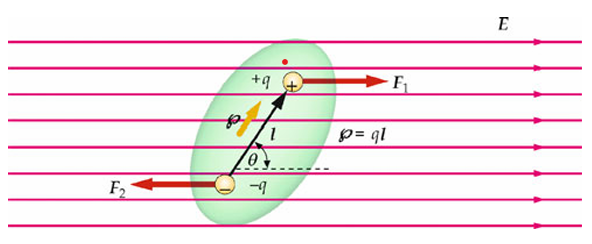
\includegraphics[width=0.5\linewidth]{Abbildungen Physik ZF/Dipol_Drehmoment.png}
\]
Das Drehmoment hat für jede der beiden Punktladungen des Dipols den Betrag:
\[
    |\Vec{F}||\Vec{l}|\sin{\theta} = |q \cdot \Vec{E}||\Vec{l}|\sin{\theta} = |\Vec{p}||\Vec{E}|\sin{\theta}
\]
In \textbf{Vektorform} gilt das \textbf{Kreuzprodukt}:
\begin{formulabox}
\[
    \Vec{M} = \Vec{p} \times \Vec{E}
\]
\end{formulabox}
Bei einer Drehung wird \textbf{Arbeit} verrichtet:
\[
    dW = - |\Vec{M}|d\theta = -|\Vec{p}||\Vec{E}|\sin{\theta}d\theta
\]\[
    dE_{pot} = -dW = |\Vec{p}||\Vec{E}|\sin{\theta}d\theta
\]
\textbf{Potentielle Energie} eins Dipols im $\Vec{E}-Feld$
\begin{formulabox}
\[
    E_{pot} = -|\Vec{p}||\Vec{E}|\cos{\theta} = -\Vec{p}\Vec{E}
\]
\end{formulabox}

\end{flushleft}